% Compiling this file requires that you have AMS-LaTeX 2.0 installed
% as well as the rest of the prerequisites for REVTeX 4.0
%
%  1)  latex summary.tex
%  2)  bibtex summary
%  3)  latex summary.tex
%  4)  latex summary.tex
%
\documentclass[prb,preprintnumbers,amsmath,amssymb, 10pt]{revtex4}

\usepackage{amsmath,amsthm,amssymb}
\usepackage{graphicx}
\usepackage{dcolumn}
\usepackage{bm}
\usepackage{color}
\usepackage{epsfig}
\usepackage{multirow}
\usepackage{mathrsfs}
\usepackage{hyperref}
\usepackage{cleveref}
\usepackage{epstopdf}
\usepackage{subcaption}
\usepackage{autobreak}
\usepackage{tikz}
\usepackage{svg}
\usepackage{placeins}

%Macros for mathematical notations
\newcommand{\V}[1]{\boldsymbol{#1}}
\newcommand{\M}[1]{\boldsymbol{#1}}
\newcommand{\Set}[1]{\mathbb{#1}}
\newcommand{\D}[1]{\Delta#1}
\renewcommand{\d}[1]{\delta#1}
\newcommand{\norm}[1]{\left\Vert #1\right\Vert }
\newcommand{\abs}[1]{\left|#1\right|}

\newcommand{\grad}{\M{\nabla}}
\newcommand{\av}[1]{\left\langle #1\right\rangle }

\newcommand{\sM}[1]{\M{\mathcal{#1}}}
\newcommand{\dprime}{\prime\prime}
\newcommand{\follows}{\quad\Rightarrow\quad}
\newcommand{\eqd}{\overset{d}{=}}
\newcommand{\spe}[1]{\mathscr{#1}}
\newcommand{\eps}{\epsilon}
\newcommand{\bra}[1]{\left\langle #1 \right|}
\newcommand{\ket}[1]{\left| #1 \right\rangle}
\newcommand{\braket}[2]{\left\langle #1 \middle| #2 \right\rangle}
\newcommand{\bracket}[3]{\left\langle #1 \middle| #2 \middle| #3 \right\rangle}

\newtheorem{theorem}{Theorem}[section]
\newtheorem{lemma}[theorem]{Lemma}
\newtheorem{definition}[theorem]{Definition}


\begin{document}
\preprint{Preprint}

\title{Summary: A Boundary-Integral Poisson Solver for Four-Index Integrals
with Dielectric Mismatches and Edge/Corner Singularities}
\author{Xuanzhao Gao}

\begin{abstract}
We summarize the problem formulation, solver, and numerical results developed
in the series of notes (\texttt{fock}, \texttt{model}, \texttt{orbital},
\texttt{cross\_interface}, \texttt{slides}).  The target is the four-index
electron-repulsion integral that drives Hartree--Fock / post-HF electronic
structure, evaluated in the presence of screening dielectric bodies with
sharp edges and corners.  We reduce the Poisson problem with piecewise
constant permittivity to a Fredholm integral equation of the second kind
for a single-layer charge density on the dielectric interfaces, and solve
it with an adaptively refined high-order Nystr\"om discretization.  The
solver exhibits exponential convergence in 2D and 3D, handles orbital
(Wannier) source data, captures the theoretically predicted corner blowup
of the single-layer density, and reproduces constrained RPA screened
interaction parameters for graphene.
\end{abstract}

\maketitle

\section{Problem Formulation}

\subsection{From Hartree--Fock to a four-index integral}

Under the Born--Oppenheimer approximation, the $N$-electron Hamiltonian is
\begin{equation}
    \hat{H} = \sum_{i=1}^N \left( -\tfrac{1}{2} \nabla_{i}^2
        - \sum_{A} \frac{Z_A}{\abs{\V{r}_i - \V{R}_A}} \right)
        + \sum_{i < j} \frac{1}{|\V{r}_i - \V{r}_j|}.
\end{equation}
Expanding the molecular orbitals $\psi_i(\V{r}) = \sum_\nu C_{\nu i}
\varphi_\nu(\V{r})$ in a basis of atomic orbitals and imposing the Slater
determinant ansatz yields the Roothaan
equation~\cite{roothaan1951new,cramer2013essentials}
$\det(\V{F}-\V{S}\V{\epsilon}) = 0$, whose Fock matrix
\begin{equation}
    F_{\mu\nu} = h_{\mu\nu} + \sum_{\lambda\sigma}\sum_i 2 C_{\lambda i} C_{\sigma i}
    \bigl( J_{\mu\nu\lambda\sigma} - \tfrac{1}{2} K_{\mu\nu\lambda\sigma} \bigr)
\end{equation}
is dominated by the Coulomb and exchange four-index integrals
\begin{equation}
    \begin{split}
    V_{ijkl} &= \iint \varphi_i(x_1)\varphi_j^*(x_1)\, K(x_1,x_2)\,
        \varphi_k(x_2)\varphi_l^*(x_2)\, \mathrm{d}x_1\mathrm{d}x_2\\
    &= \int \rho_{ij}(x_1)\, \phi_{kl}(x_1)\, \mathrm{d}x_1,
    \end{split}
\end{equation}
with pair density $\rho_{ij}(x) = \varphi_i(x)\varphi_j^*(x)$ and potential
$\phi_{kl}(x)$.  With $\mathcal{O}(10^4)$ basis functions and formal
$\mathcal{O}(N^4)$ scaling, fast and accurate evaluation of $\phi_{kl}$ in the
presence of nearby dielectric bodies is the central computational bottleneck.

\subsection{Poisson problem with piecewise constant dielectric}

We target the geometry in Fig.~\ref{fig:system}: a material region
$\Omega_m$ containing the source densities, embedded near one or several
dielectric slabs/boxes $\Omega_1, \Omega_2, \dots$, with vacuum $\Omega_0$
outside.  The permittivity is piecewise constant,
\begin{equation}
    \epsilon(x) = \begin{cases}
        \epsilon_m, & x \in \Omega_m,\\
        \epsilon_k, & x \in \Omega_k,\ k=1,2,\dots,\\
        \epsilon_0 = 1, & x \in \Omega_0,
    \end{cases}
\end{equation}
and the potential solves $\grad_x \cdot (\epsilon(x) \grad_x \phi(x)) =
-\rho(x)$, which is equivalent to the boundary-value problem
\begin{equation}\label{eq:bvp}
    \begin{cases}
        \epsilon_m \Delta_x \phi(x) = -\rho(x), & x \in \Omega_m,\\
        \Delta_x \phi(x) = 0, & x \notin \Omega_m,\\
        \phi\mid_{\partial \Omega_i} = \phi\mid_{\partial \Omega_j}, &
            x \in \partial\Omega_i \cap \partial\Omega_j,\\
        \epsilon_i \partial_{\V n} \phi\mid_{\partial \Omega_i}
            = \epsilon_j \partial_{\V n} \phi\mid_{\partial \Omega_j}, &
            x \in \partial\Omega_i \cap \partial\Omega_j,\\
        \phi(x) \to 0, & \abs{x} \to \infty.
    \end{cases}
\end{equation}

\begin{figure}[htbp]
    \centering
    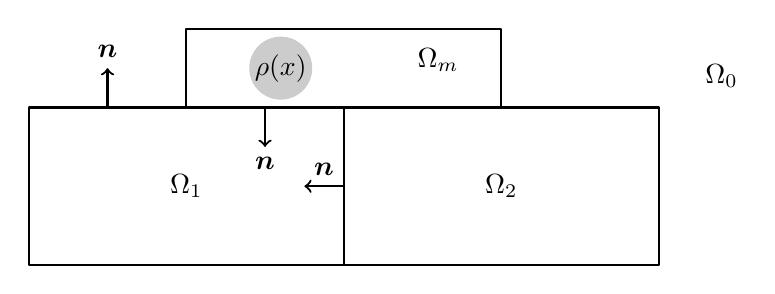
\begin{tikzpicture}[scale=1.0, line join=round, line cap=round]
      \def\s{4.0}
      \def\h{2.0}
      \coordinate (A) at (0,0); \coordinate (B) at (\s,0);
      \coordinate (C) at (\s,\h); \coordinate (D) at (0,\h);
      \coordinate (E) at (\s, 0); \coordinate (F) at (2*\s, 0);
      \coordinate (G) at (2*\s, \h); \coordinate (H) at (\s, \h);
      \coordinate (I) at (0.5*\s, 1.5*\h); \coordinate (J) at (1.5*\s, 1.5*\h);
      \coordinate (K) at (1.5*\s, \h); \coordinate (L) at (0.5*\s, \h);
      \draw[thick] (A)--(B)--(C)--(D)--cycle;
      \draw[thick] (E)--(F)--(G)--(H)--cycle;
      \draw[thick] (I)--(J)--(K)--(L)--cycle;
      \node at (1.3*\s, 1.3*\h) {$\Omega_m$};
      \node at (\s/2, \h/2) {$\Omega_1$};
      \node at (1.5*\s, \h/2) {$\Omega_2$};
      \node at (2.2*\s, 1.2*\h) {$\Omega_0$};
      \coordinate (S) at (0.8*\s, 1.25*\h);
      \fill[gray, opacity=0.4] (S) circle (0.2*\h);
      \node at (S) {$\rho(x)$};
      \draw[->, thick] (\s/4,\h) -- (\s/4,\h+0.5) node[right,above] {$\V n$};
      \draw[->, thick] (\s,\h/2) -- (\s-0.5,\h/2) node[midway,above] {$\V n$};
      \draw[->, thick] (\s*3/4,\h) -- (\s*3/4,\h-0.5) node[right,below] {$\V n$};
    \end{tikzpicture}
    \caption{2D cartoon of the system geometry.  The gray blob is the
      source density $\rho(x)$ supported in the material region $\Omega_m$;
      $\Omega_{1,2}$ are dielectric slabs; the remainder is vacuum $\Omega_0$.
      Arrows indicate the outward normal on each interface.}
    \label{fig:system}
\end{figure}

\section{Solver}

\subsection{Reduction to a single-layer integral equation}

We split the potential as $\phi = u_{\text{inc}} + u$, with the free-space
incident potential
\begin{equation}
    u_{\text{inc}}(x) = \frac{1}{4\pi\epsilon_m}
        \int \frac{\rho(x')}{\abs{x-x'}}\, \mathrm{d}x',
\end{equation}
and a single-layer representation of the scattered field on the union
$\Gamma$ of dielectric interfaces,
\begin{equation}
    u(x) = \frac{1}{4\pi}\int_\Gamma \frac{\sigma(x')}{\abs{x-x'}}\, \mathrm{d}S(x').
\end{equation}
Using the standard jump relation $\partial_{\V n} u(\V r^{\pm}) = D^T\sigma(x)
\mp \tfrac{1}{2}\sigma(x)$, the interfacial flux-matching condition in
\eqref{eq:bvp} reduces to the Fredholm integral equation of the second
kind~\cite{greengard1994numerical}
\begin{equation}\label{eq:sl}
    \tfrac{1}{2}\frac{\epsilon_i+\epsilon_j}{\epsilon_i-\epsilon_j}\sigma(x)
        + D^T \sigma(x) = -\partial_{\V n} u_{\text{inc}}(x),
        \qquad x \in \partial\Omega_i \cap \partial\Omega_j,
\end{equation}
which is identical to Eq.~(2.19) of Ref.~\cite{greengard1994numerical}.

\subsection{Algorithm}

The four steps of the solver are:
\begin{enumerate}
  \item[1.] Build the source density $\rho$ (point charge, Gaussian, or a
      product of Wannier functions read from \texttt{.xsf} files), and
      evaluate $\partial_{\V n} u_{\text{inc}}$ on the discretized
      interface.
  \item[2.] Discretize $\Gamma$ into panels with $p\times p$ tensor-product
      Gauss--Legendre nodes, refined dyadically toward edges, corners, and
      toward regions where the source density is close to the boundary.
  \item[3.] Assemble a discrete representation of $D^T$; evaluate the
      non-self interactions through FMM2D/FMM3D for scalability.
  \item[4.] Solve \eqref{eq:sl} by GMRES to obtain $\sigma$, then evaluate
      $\phi = u_{\text{inc}} + u$ at arbitrary target points and contract
      against $\rho_{ij}$ to produce $V_{ijkl}$.
\end{enumerate}

\subsection{Handling orbital densities across interfaces}

When a Wannier/orbital density $\rho$ crosses a dielectric interface, the
``screened'' density $\tilde\rho(y) = \rho_i(y)/\epsilon_i$ used inside
$u_{\text{inc}}$ is \emph{discontinuous}, so its Fourier transform decays
slowly and defeats the TKM--Fourier evaluator (Fig.~\ref{fig:screened-ft}).
Because the physical permittivity cannot change sharply on atomic scales,
we smooth $\epsilon$ through the interface using an $\text{erf}$-type
transition $P(x)$, with two natural choices,
\begin{equation}
    \tilde\epsilon(x) = \epsilon_1 P(x) + \epsilon_2 (1-P(x)),
    \quad\text{or}\quad
    \tilde\epsilon(x) = \bigl[ P(x)/\epsilon_1 + (1-P(x))/\epsilon_2 \bigr]^{-1}.
\end{equation}
To avoid also smoothing the boundary-integral kernel we use a \emph{hybrid}
model: the incident potential $u_{\text{inc}}^{\prime}$ is computed with
smooth $\tilde\epsilon$ (fast-decaying Fourier, amenable to TKM), while the
single-layer equation \eqref{eq:sl} is retained with the original sharp
interface.  The smoothing bandwidth is a physical parameter tunable against
ab initio / experimental pair interactions.

\subsection{Corner singularities, conditioning, and near-field evaluation}

Edges and corners of the dielectric boxes produce integrable singularities
in $\sigma$ of the form $\sigma(x) = \mathcal{O}(x^k)$, with $k$ a function
of the contrast $\gamma = (1-\epsilon_m)/(1+\epsilon_m)$ that matches the
theory of Ref.~\cite{van2007electromagnetic}; dyadic panel refinement
resolves this blowup and restores exponential convergence.  The largest
eigenvalue of $D^T$ is exactly $1/2$, so \eqref{eq:sl} is ill-conditioned as
$\epsilon_m \to \infty$ (perfect conductor limit); GMRES iteration counts
grow but remain moderate in practice.  For nearby targets (high aspect
ratio slabs, orbitals near interfaces) we quantify and control quadrature
error via Bernstein-ellipse estimates~\cite{trefethen2019approximation}:
for a pole at $z = x_0 + i y_0$ the $p$-point Gauss--Legendre error decays
as $\rho(z)^{-2p}$, where
$\rho(z) = \max(\abs{z\pm\sqrt{z^2-1}})$.  In 3D we combine two 2D
estimates via $\rho_{3D} = \min(\rho_x,\rho_y)$ and use upsampling of the
source representation to regain accuracy when $\rho_{3D}$ is close to $1$.

\section{Numerical Results}

\subsection{2D: single and multiple boxes}

For a single 2D dielectric box with a point charge, non-adaptive
discretization stalls at low accuracy when the charge is close to the
boundary (Fig.~\ref{fig:2d-nonadapt}).  With dyadic corner refinement the
self-convergence error decays exponentially in both quadrature order $p$
and adaptation depth $n_{\text{adapt}}$, reaching machine precision
(Fig.~\ref{fig:2d-adapt}).  A drop in accuracy is observed as
$\gamma\to 1$, consistent with the loss of conditioning of $D^T$.
The fitted corner blowup rate $k(\gamma)$ agrees with the theoretical
spectrum of Ref.~\cite{van2007electromagnetic}, and at
$\gamma=\pm 1$ we recover $k=-1/3$
(Fig.~\ref{fig:2d-blowup}).

\begin{figure}[htbp]
    \centering
    \includesvg[width=0.45\linewidth]{../codes/box2d/figs/convergence_nonadaptive.svg}
    \caption{2D single box, non-adaptive: slow convergence when the source
        is near the boundary.}
    \label{fig:2d-nonadapt}
\end{figure}

\begin{figure}[htbp]
    \centering
    \includesvg[width=0.9\linewidth]{../codes/box2d/figs/convergence_adaptive.svg}
    \caption{2D single box, adaptive corner refinement: exponential
        convergence to machine precision in both $p$ and $n_{\text{adapt}}$.}
    \label{fig:2d-adapt}
\end{figure}

\begin{figure}[htbp]
    \centering
    \begin{subfigure}[c]{0.58\linewidth}
        \includesvg[width=\linewidth]{../codes/box2d/figs/blowup_rate.svg}
    \end{subfigure}
    \hfill
    \begin{subfigure}[c]{0.4\linewidth}
        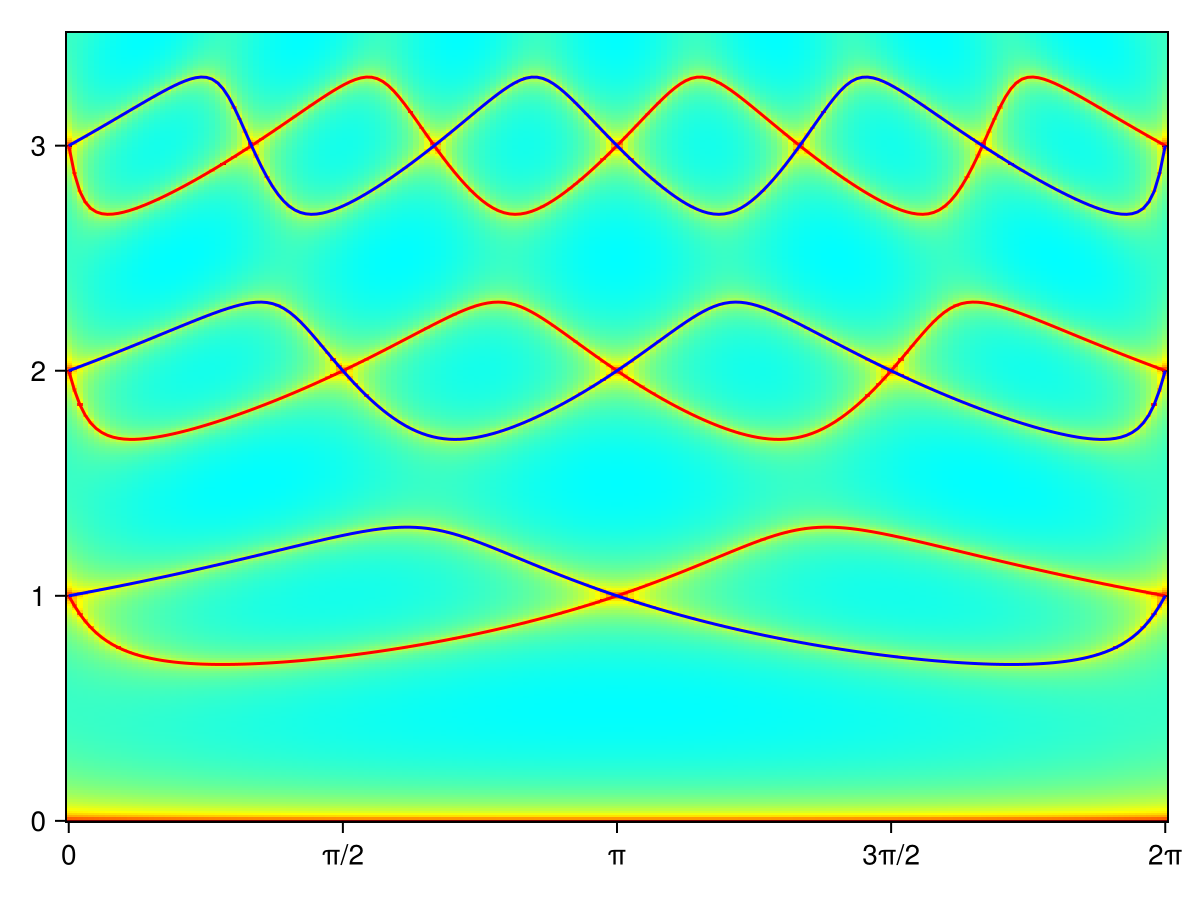
\includegraphics[width=\linewidth]{../codes/box2d/figs/blowup_rate_compare.png}
    \end{subfigure}
    \caption{Corner blowup rate $k(\gamma)$ for the 2D single box; the
        fitted data (left) follow the theoretical spectrum (right) of
        Ref.~\cite{van2007electromagnetic}.}
    \label{fig:2d-blowup}
\end{figure}

\begin{figure}[htbp]
    \centering
    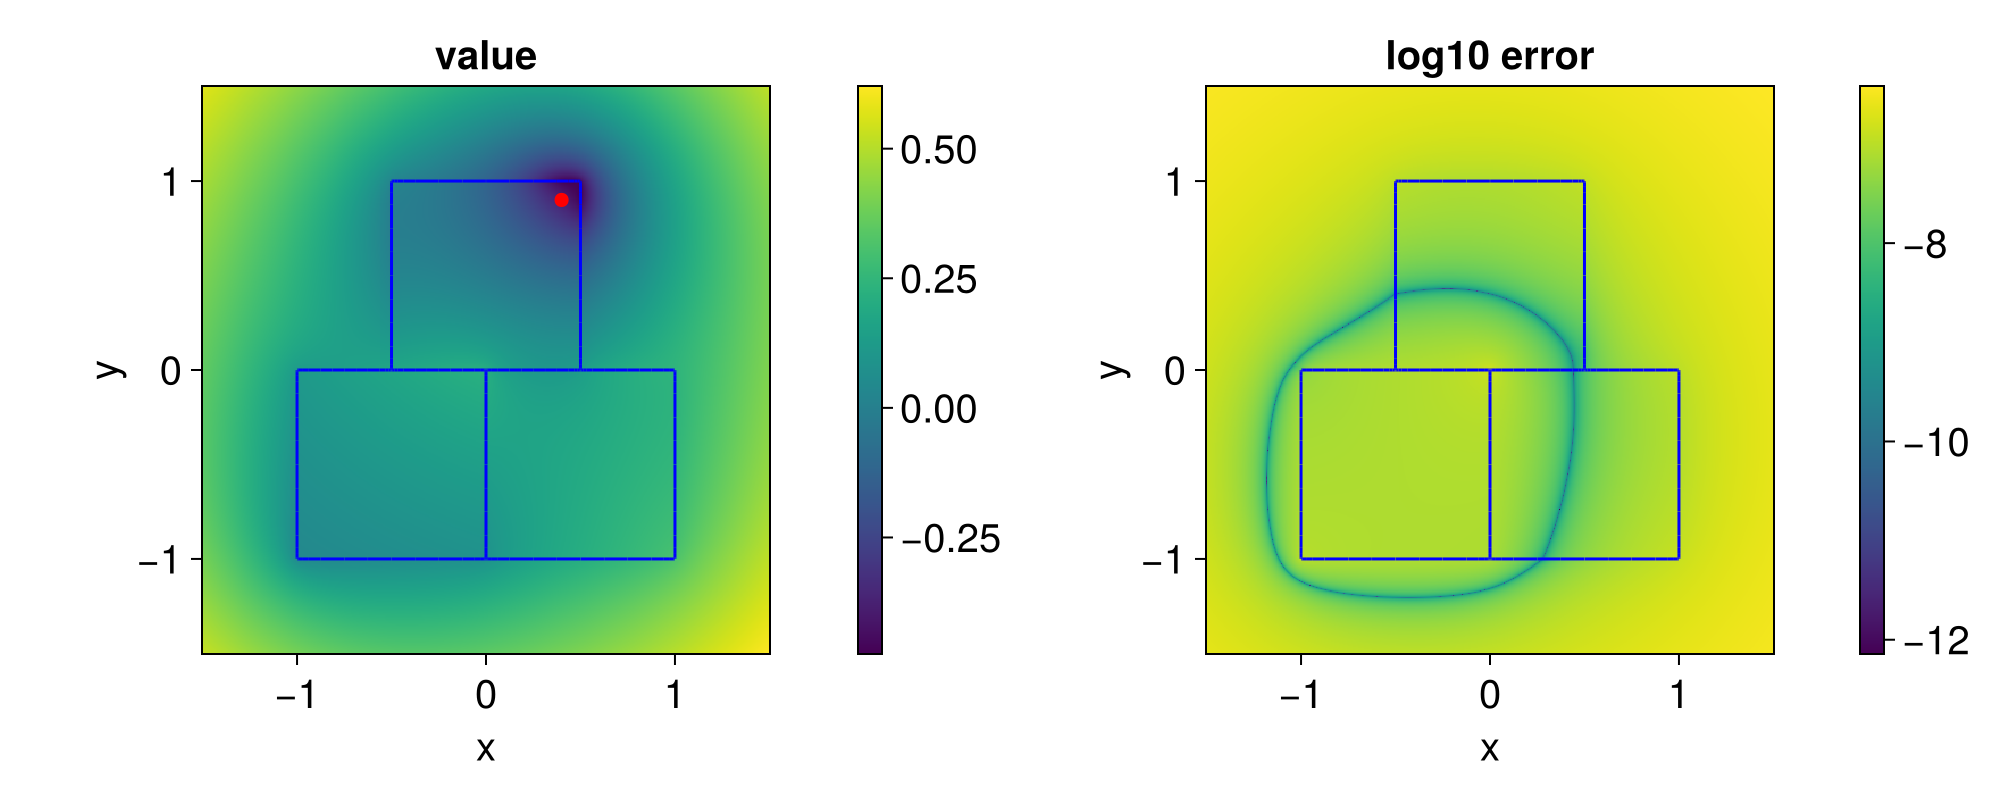
\includegraphics[width=0.8\linewidth]{../codes/box2d/figs/mbox_fmm2d_3.png}
    \caption{Potential and error for three 2D boxes with
        $\epsilon_1=100$, $\epsilon_2=3$, $\epsilon_m=4$.  Reference is
        $n_{\text{adapt}}=30$.}
    \label{fig:2d-mbox}
\end{figure}

\begin{figure}[htbp]
    \centering
    \includesvg[width=0.9\linewidth]{../codes/box2d/figs/convergence_mbox.svg}
    \caption{Convergence for the multi-box 2D configuration, same dyadic
        adaptive strategy.}
    \label{fig:2d-mbox-conv}
\end{figure}

Multi-box configurations (Fig.~\ref{fig:2d-mbox}) converge at the same
exponential rate (Fig.~\ref{fig:2d-mbox-conv}).  The condition number and
GMRES iteration count both grow with $\epsilon_m$, with the largest
eigenvalue of $D^T$ pinned at $1/2$, consistent with the ill-conditioning
argument above.

\subsection{3D: single, double, and high-aspect-ratio boxes}

In 3D we compare three surface discretizations (Fig.~\ref{fig:3d-disc}):
(a)~non-adaptive with large $p$, (b)~adaptive with fixed $p$, and
(c)~adaptive with $p$ gradually reduced near edges and corners.  The
Green's identity $D\,1 = -\tfrac{1}{2}$ is used as a mesh-quality check
(Fig.~\ref{fig:3d-gi}).

\begin{figure}[htbp]
    \centering
    \begin{subfigure}[b]{0.3\textwidth}
        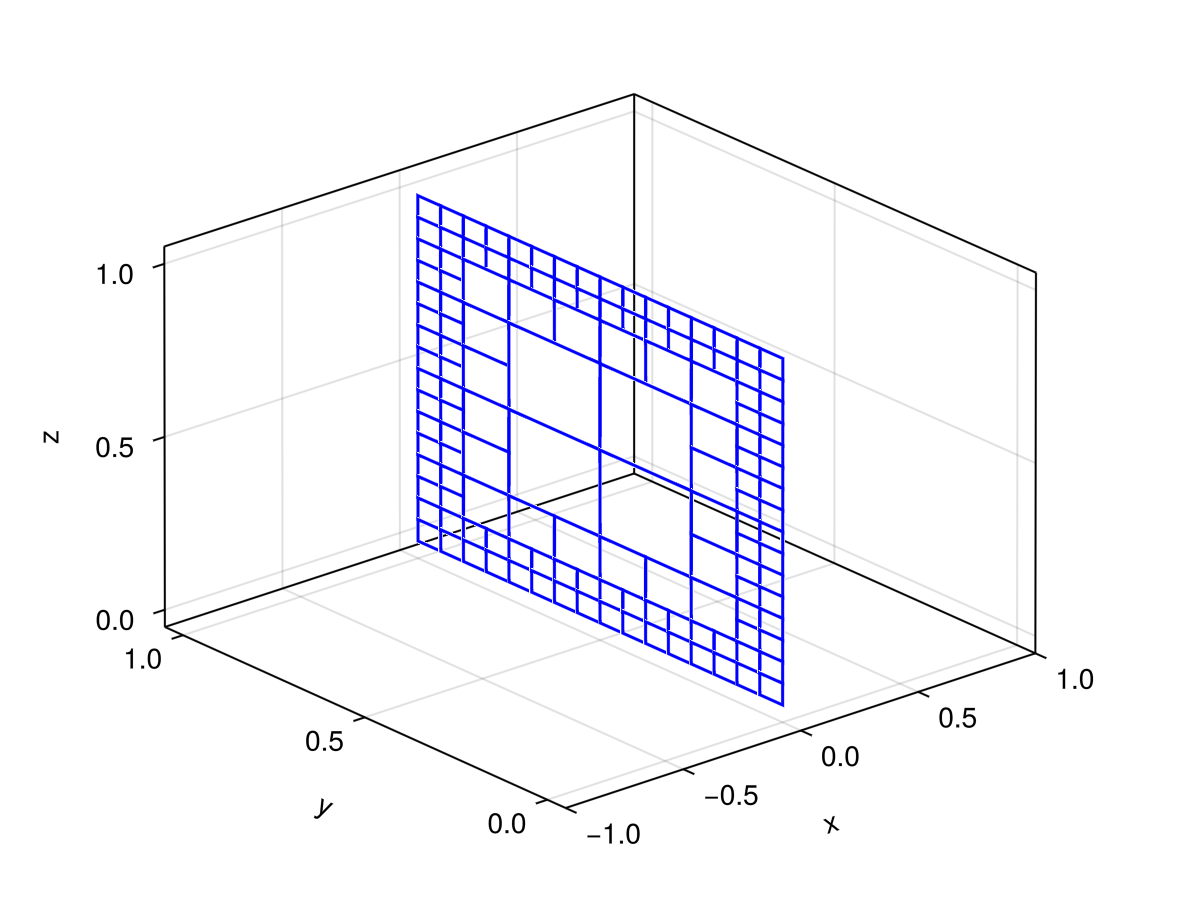
\includegraphics[width=\linewidth]{figs/squares.png}
    \end{subfigure}
    \begin{subfigure}[b]{0.3\textwidth}
        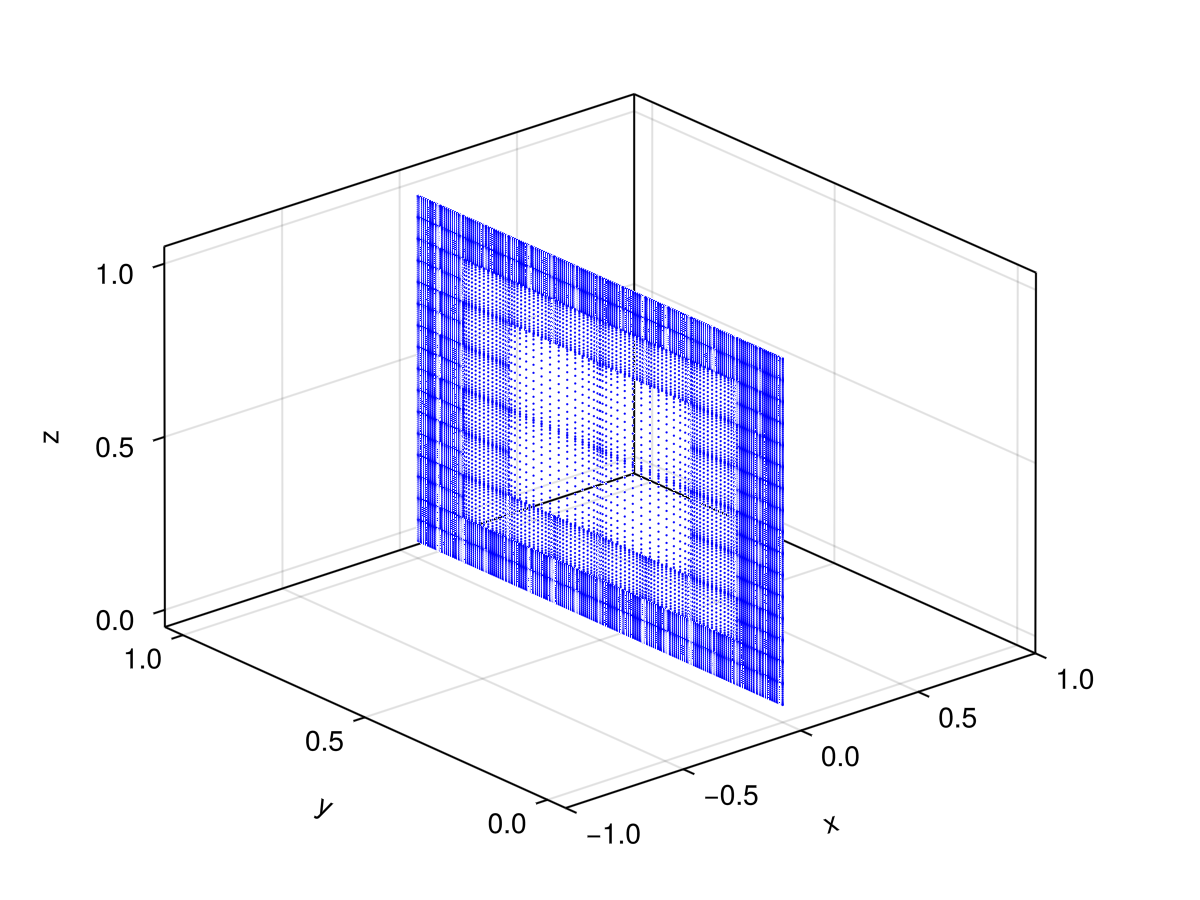
\includegraphics[width=\linewidth]{figs/discretization.png}
    \end{subfigure}
    \begin{subfigure}[b]{0.3\textwidth}
        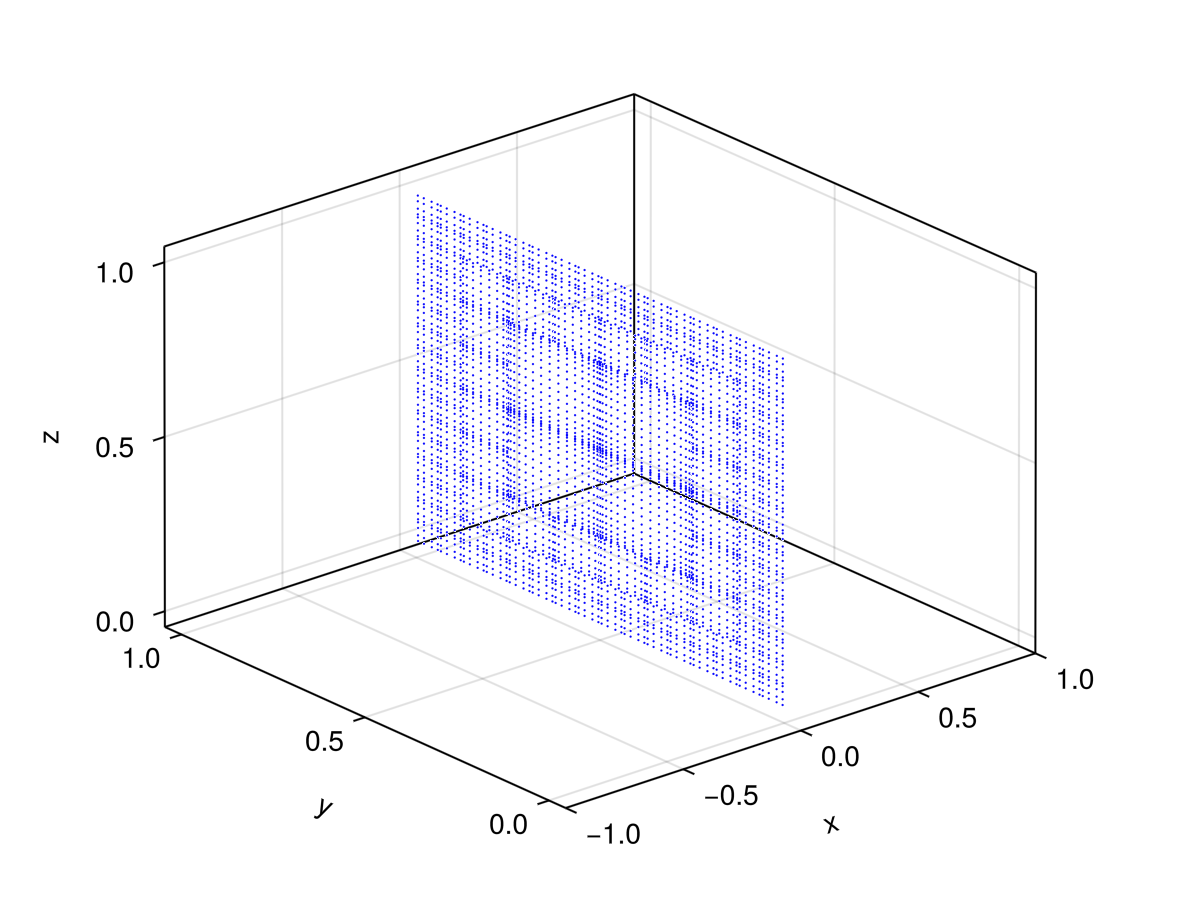
\includegraphics[width=\linewidth]{figs/reduced_discretization.png}
    \end{subfigure}
    \caption{3D surface discretization strategies: (a) panels only,
        (b) fixed $p$ per panel, (c) $p$ reduced near edges/corners.}
    \label{fig:3d-disc}
\end{figure}

\begin{figure}[htbp]
    \centering
    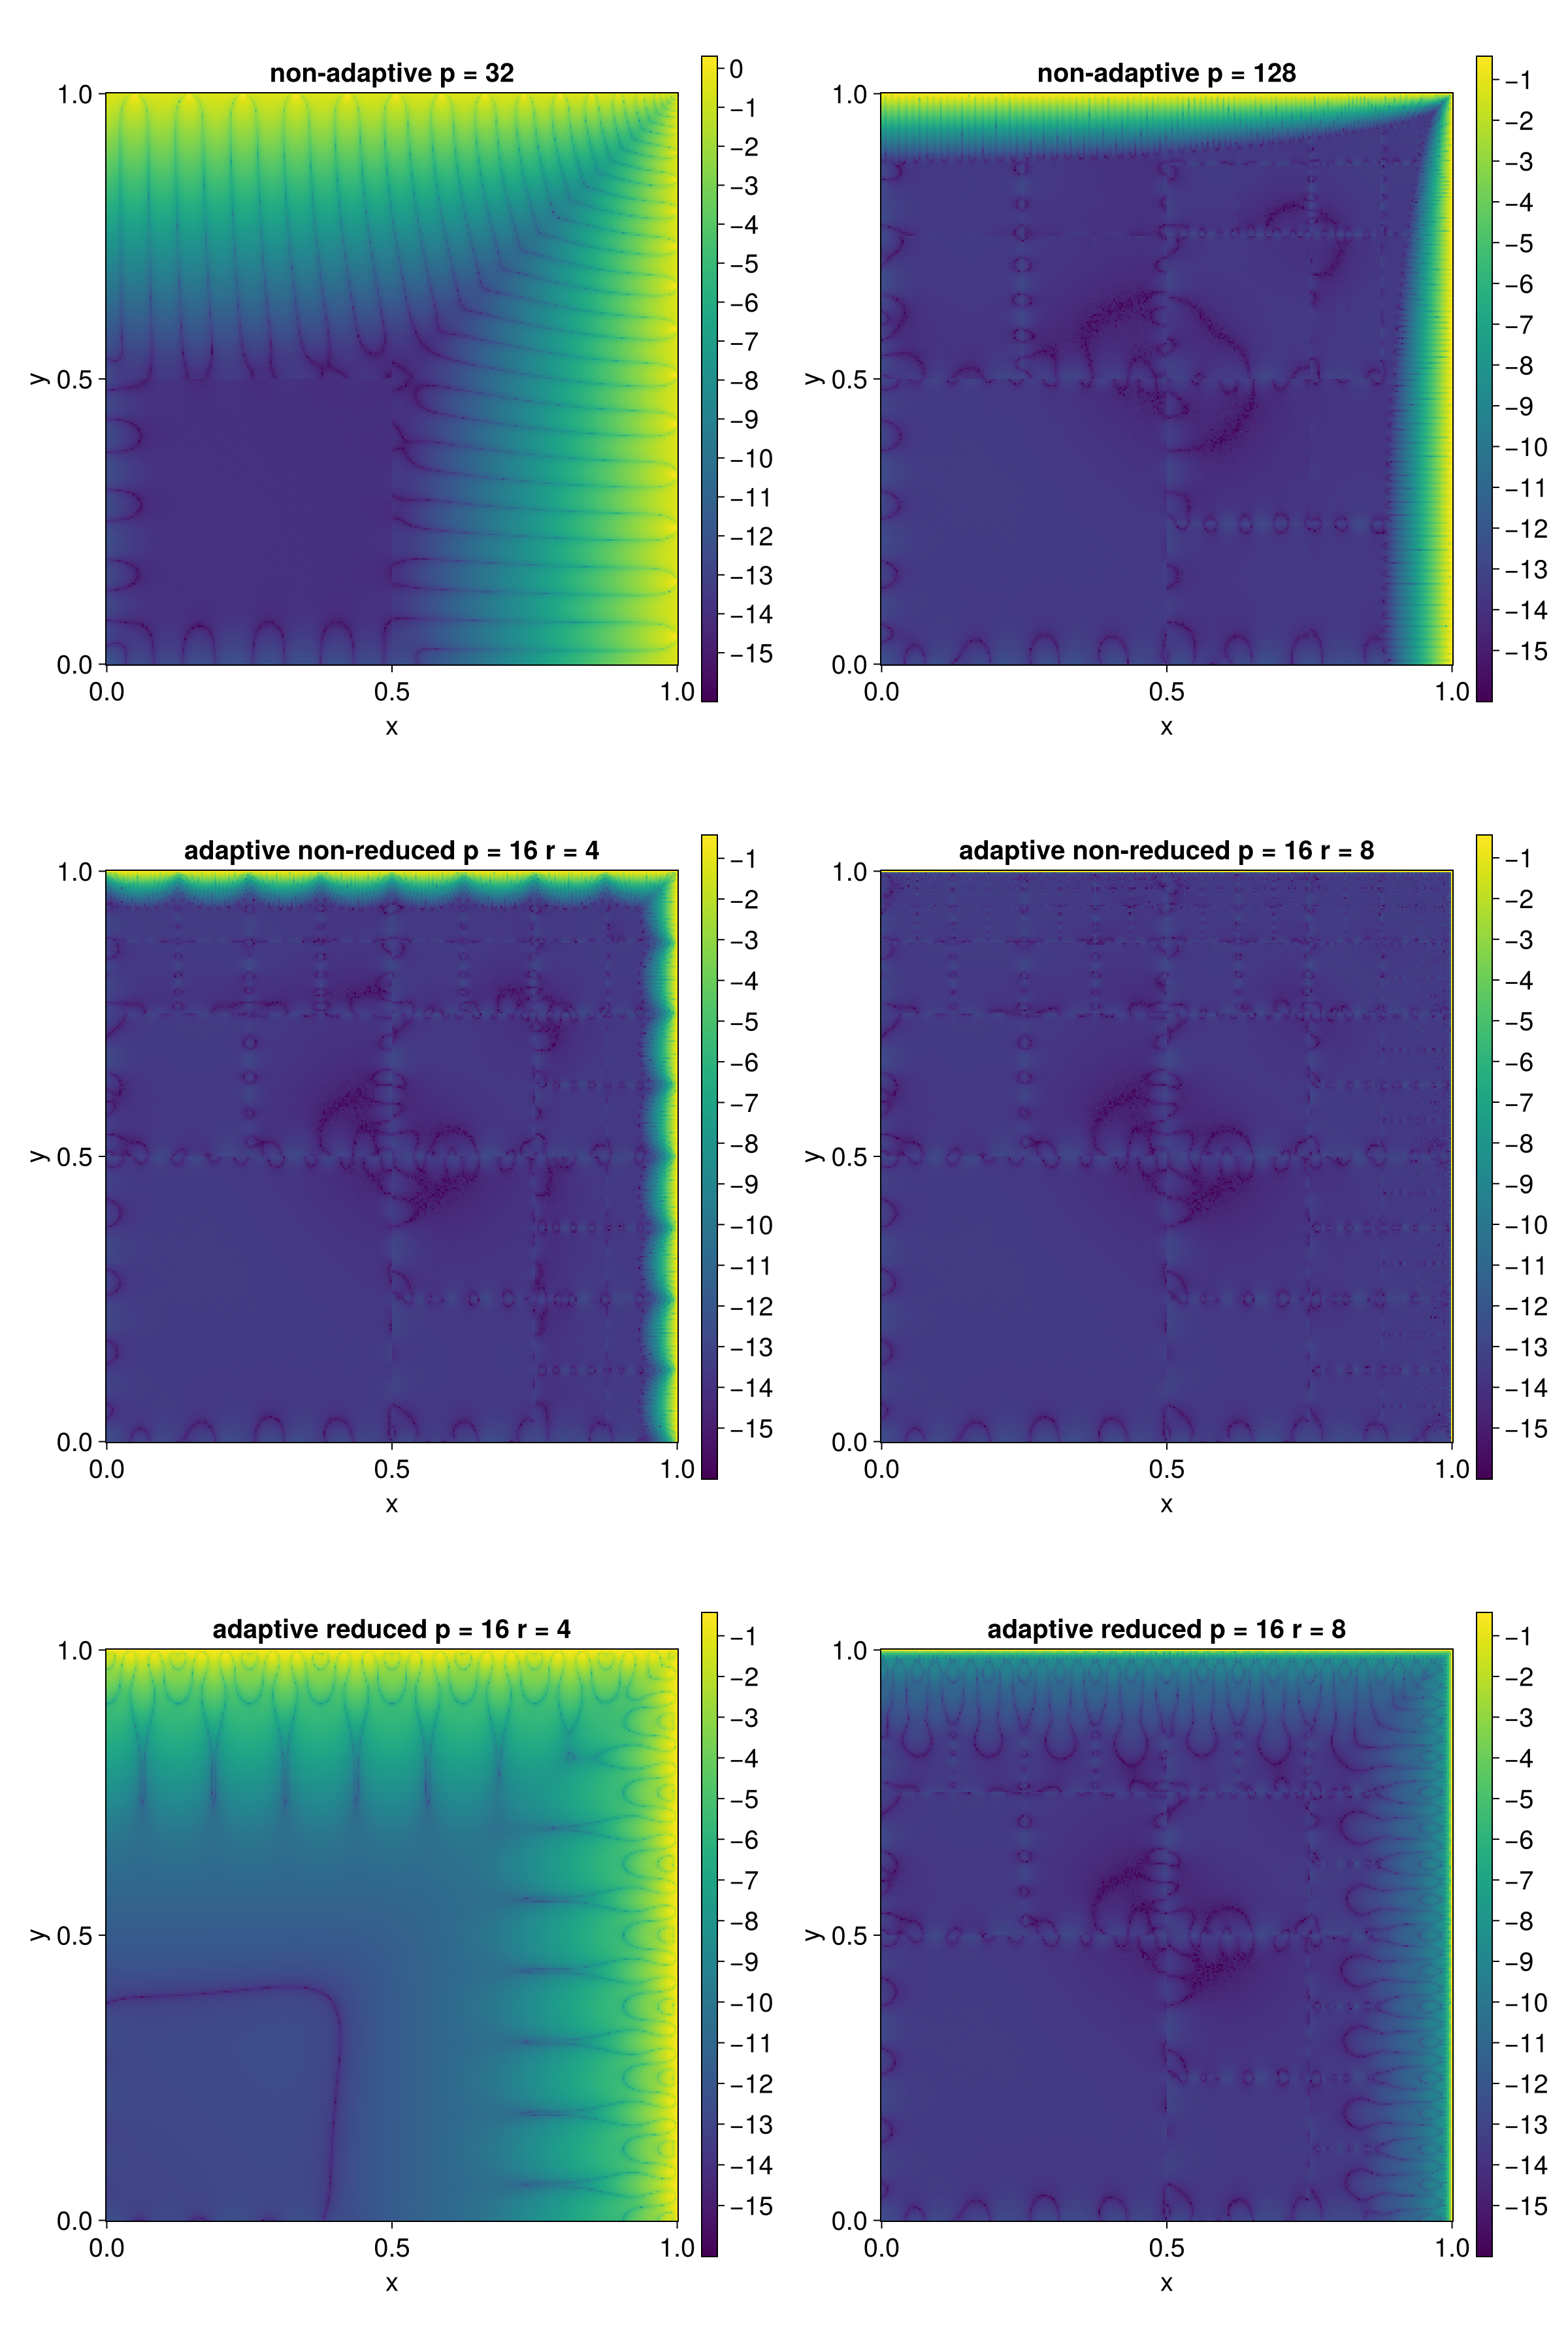
\includegraphics[width=0.8\linewidth]{../codes/box3d/figs/single_box3d_gi_heatmap.png}
    \caption{Error in Green's identity $D\,1=-1/2$ across the three
        strategies; FMM3D is used for far evaluation.}
    \label{fig:3d-gi}
\end{figure}

With a single cubic box ($\epsilon_m=4$, source at $(0.2,0.3,0.4)$),
non-adaptive discretization requires $p\gtrsim 16$ to converge
(Fig.~\ref{fig:3d-nonadapt}); adaptive refinement at fixed $p$ shows
exponential error decay with $n_{\text{adapt}}$, with $p$ controlling the
asymptotic plateau (Fig.~\ref{fig:3d-adapt}); the reduced-$p$ strategy
produces similar decay with the error dominated by edge panels
(Fig.~\ref{fig:3d-reduced}).  Double-box and high-aspect-ratio
configurations (Figs.~\ref{fig:3d-double}, \ref{fig:3d-aspect}) behave
analogously, but the high-aspect-ratio regime reveals the need for
explicit near-field evaluation when $L_{xy} \gg L_z$.

\begin{figure}[htbp]
    \centering
    \includesvg[width=0.8\linewidth]{../codes/box3d/figs/single_box3d_nonadapt.svg}
    \caption{3D single box, non-adaptive: potential on a sphere of
        radius~2 and total flux versus $1-\epsilon_m^{-1}$.}
    \label{fig:3d-nonadapt}
\end{figure}

\begin{figure}[htbp]
    \centering
    \includesvg[width=0.8\linewidth]{../codes/box3d/figs/single_box3d_convergence.svg}
    \caption{3D single box, adaptive with fixed $p$.  Error decays
        exponentially in $n_{\text{adapt}}$; low $p$ shows a transient
        growth before the asymptotic regime.}
    \label{fig:3d-adapt}
\end{figure}

\begin{figure}[htbp]
    \centering
    \includesvg[width=0.8\linewidth]{../codes/box3d/figs/single_box3d_reduce_convergence.svg}
    \caption{3D single box, adaptive with reduced $p$ near edges/corners.
        Edge panels dominate the residual error.}
    \label{fig:3d-reduced}
\end{figure}

\begin{figure}[htbp]
    \centering
    \includesvg[width=0.8\linewidth]{../codes/box3d/figs/double_box3d_convergence.svg}
    \caption{Two adjacent 3D cubic boxes: same convergence pattern, error
        floor set by $p$.}
    \label{fig:3d-double}
\end{figure}

\begin{figure}[htbp]
    \centering
    \includesvg[width=0.9\linewidth]{../codes/box3d/figs/single_thin_box_convergence.svg}
    \caption{High-aspect-ratio boxes ($L_z=1$, varying $L$).  Motivates
        near-field evaluation (Sec.~\ref{sec:near}).}
    \label{fig:3d-aspect}
\end{figure}

\subsection{Near-field evaluation and Bernstein ellipses}
\label{sec:near}

For nearby sources, 2D integration error follows the predicted
$\rho^{-2p}$ decay with $\rho$ the Bernstein-ellipse radius
(Fig.~\ref{fig:2d-ellipse}).  In 3D the combined estimate
$\rho_{3D} = \min(\rho_x,\rho_y)$ accurately predicts the quadrature error
(Fig.~\ref{fig:3d-ellipse}).  Upsampling the single-layer density
representation before integration extends the asymptotic regime, with
error tracking $\rho^{-2 n_{\text{up}}}$
(Fig.~\ref{fig:3d-upsample}).

\begin{figure}[htbp]
    \centering
    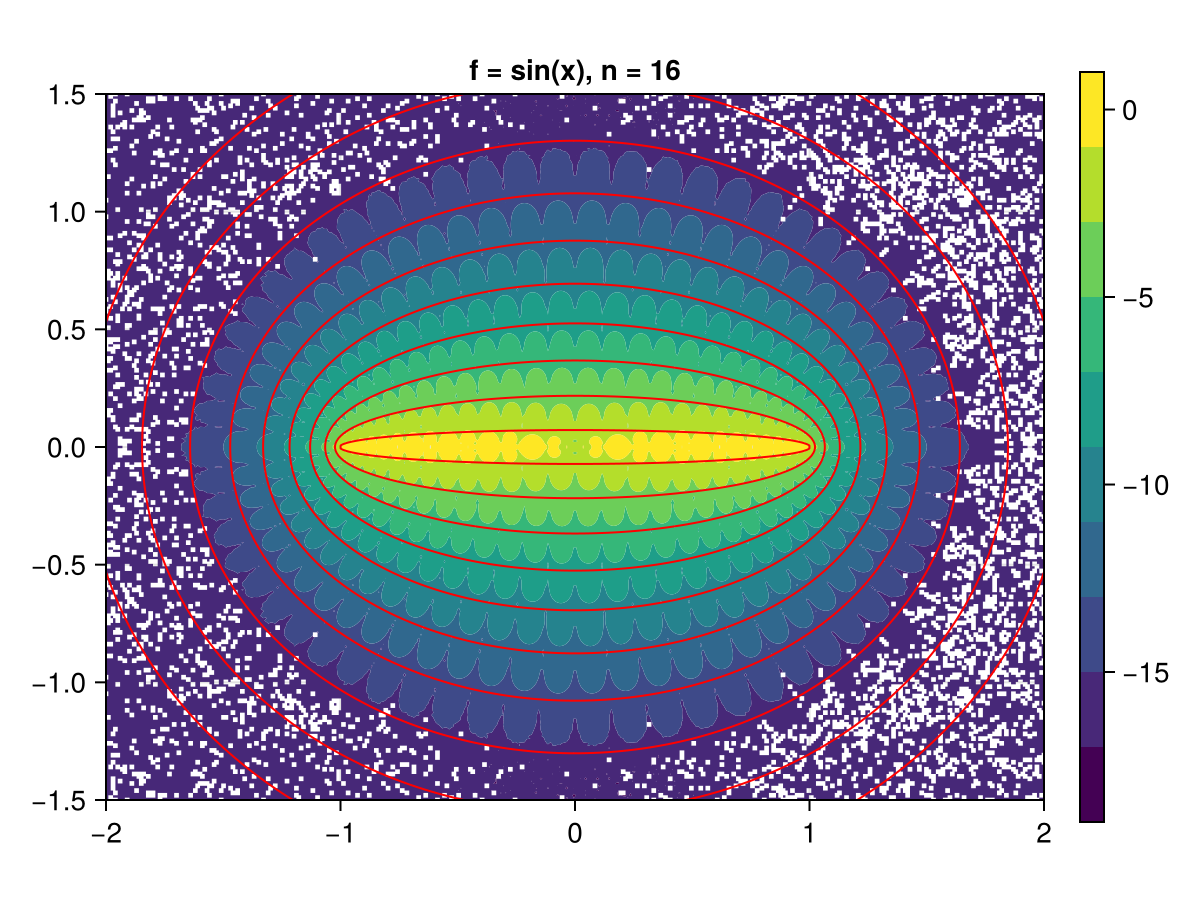
\includegraphics[width=0.55\linewidth]{../codes/bernstein_ellipses/ellipes2d_n16.png}
    \caption{2D integration error with predictions from Bernstein ellipses.}
    \label{fig:2d-ellipse}
\end{figure}

\begin{figure}[htbp]
    \centering
    \begin{subfigure}[b]{0.3\textwidth}
        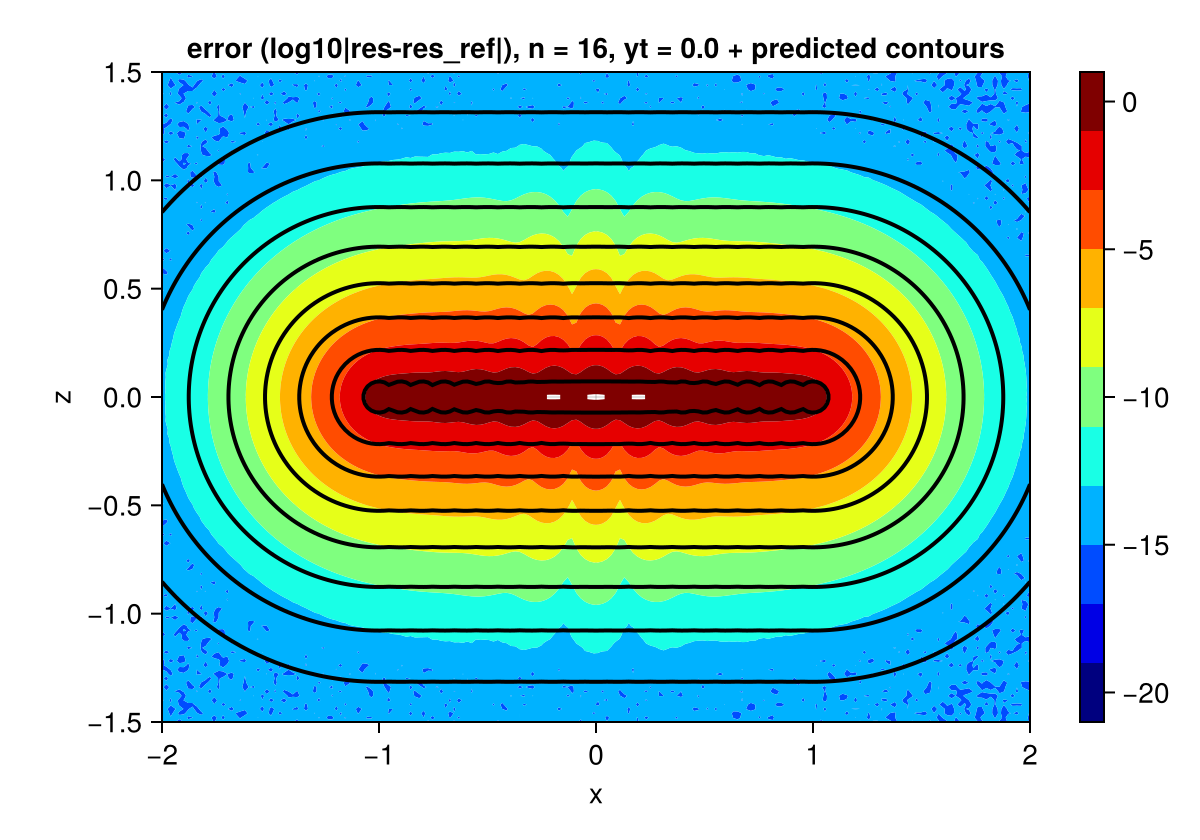
\includegraphics[width=\linewidth]{../codes/bernstein_ellipses/3d_figs/ellipes3d_overlay_n16_yt0.0.png}
    \end{subfigure}
    \begin{subfigure}[b]{0.3\textwidth}
        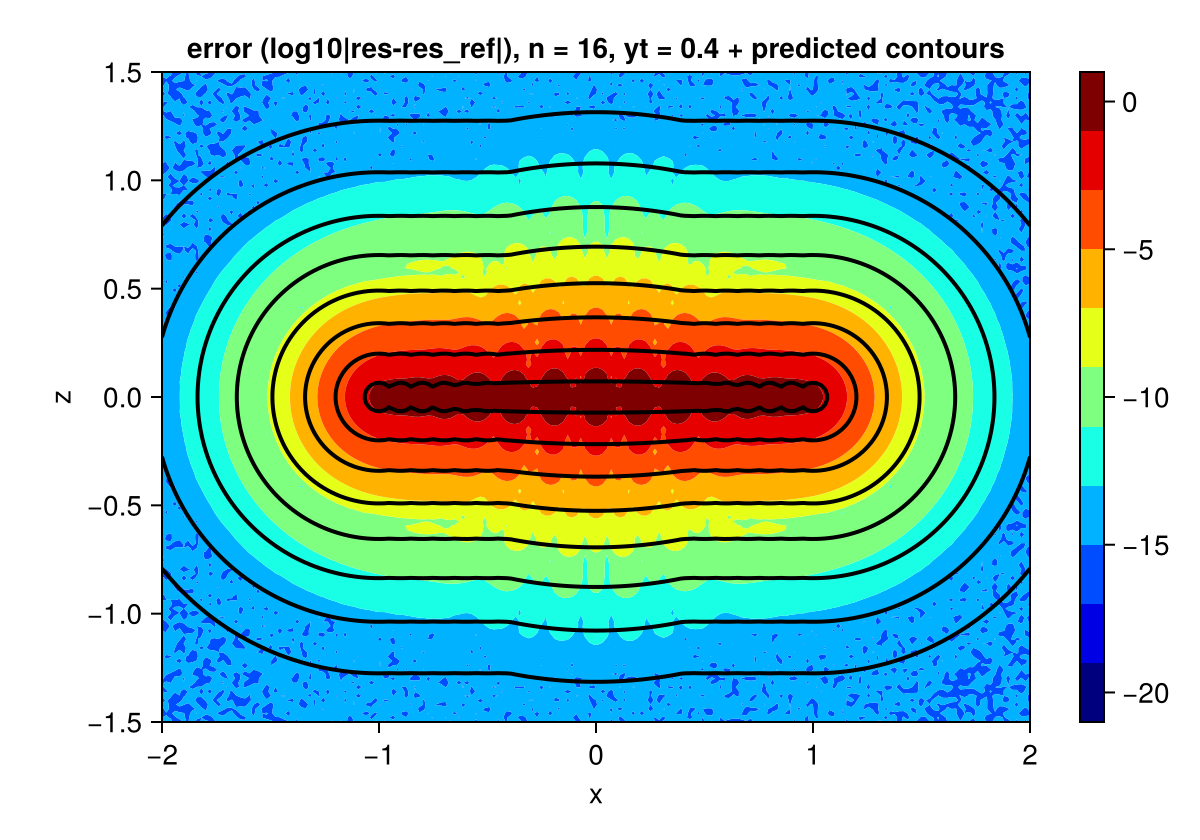
\includegraphics[width=\linewidth]{../codes/bernstein_ellipses/3d_figs/ellipes3d_overlay_n16_yt0.4.png}
    \end{subfigure}
    \begin{subfigure}[b]{0.3\textwidth}
        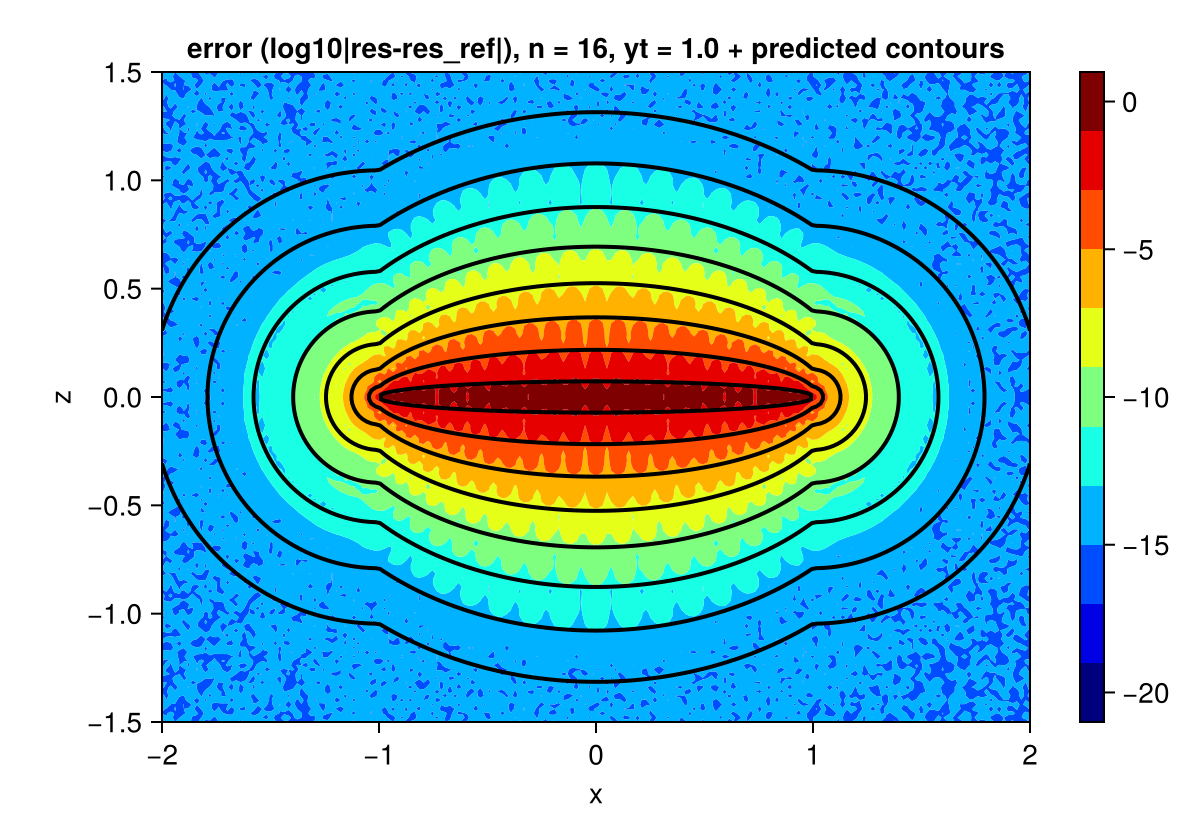
\includegraphics[width=\linewidth]{../codes/bernstein_ellipses/3d_figs/ellipes3d_overlay_n16_yt1.0.png}
    \end{subfigure}
    \caption{3D integration error in planar slices; lines are Bernstein
        predictions using $\rho_{3D}$.}
    \label{fig:3d-ellipse}
\end{figure}

\begin{figure}[htbp]
    \centering
    \includesvg[width=0.9\linewidth]{../codes/near_eval/figs/doublelayer_upsampling_error.svg}
    \caption{Double-layer density integration error on an opposite plane,
        with upsampling; black dotted lines are $\rho^{-2n_{\text{up}}}$.}
    \label{fig:3d-upsample}
\end{figure}

\subsection{Orbital (Wannier) source data: graphene}

Using Wannier functions from \texttt{graphene\_*.xsf} (shifted to atomic
centers and truncated in $z$), the product density $\rho_{ij}$ is embedded
in a $(90,90,9)$ box with $\epsilon_r = 6$, and the surface is adaptively
refined near the density, edges, and corners
(Fig.~\ref{fig:orbital-panels}).  Solving \eqref{eq:sl} yields the
surface density of Fig.~\ref{fig:orbital-sol}, and a self-convergence
study at fixed evaluation points shows exponential decay in the
edge-refinement level $l_{\min}$ at each order $p$
(Fig.~\ref{fig:orbital-conv}).

\begin{figure}[htbp]
    \centering
    \begin{subfigure}[t]{0.4\textwidth}
        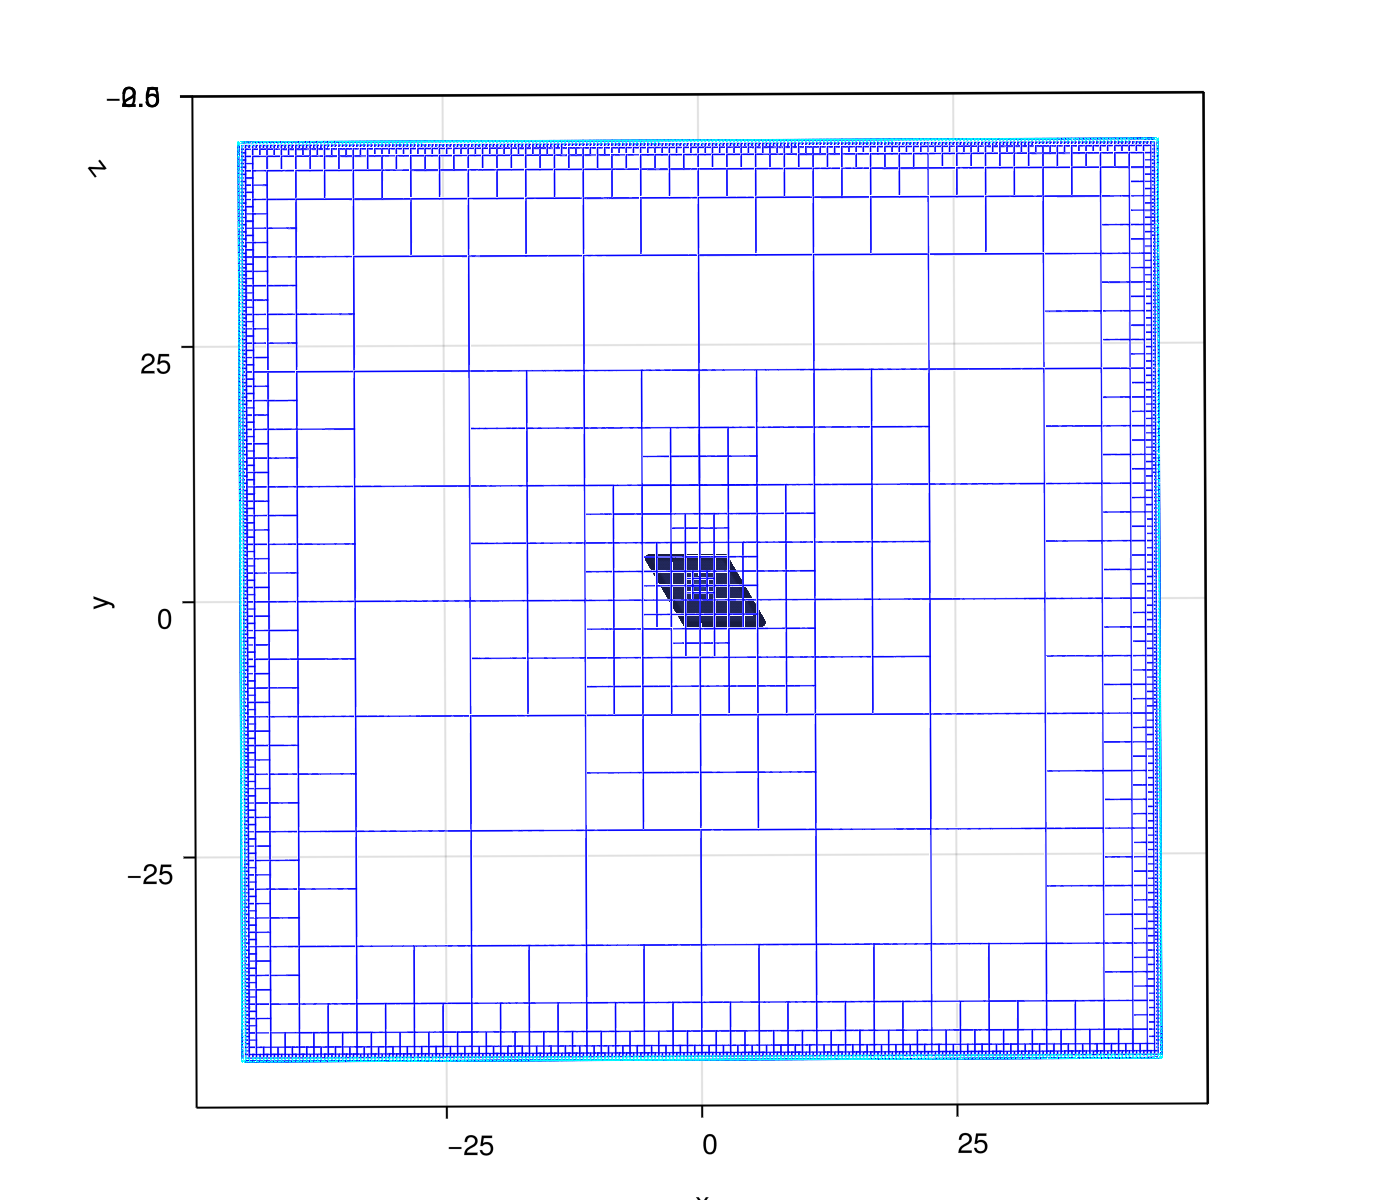
\includegraphics[width=\linewidth]{../codes/viz/figs/graphene_orbital_1.png}
    \end{subfigure}
    \begin{subfigure}[t]{0.4\textwidth}
        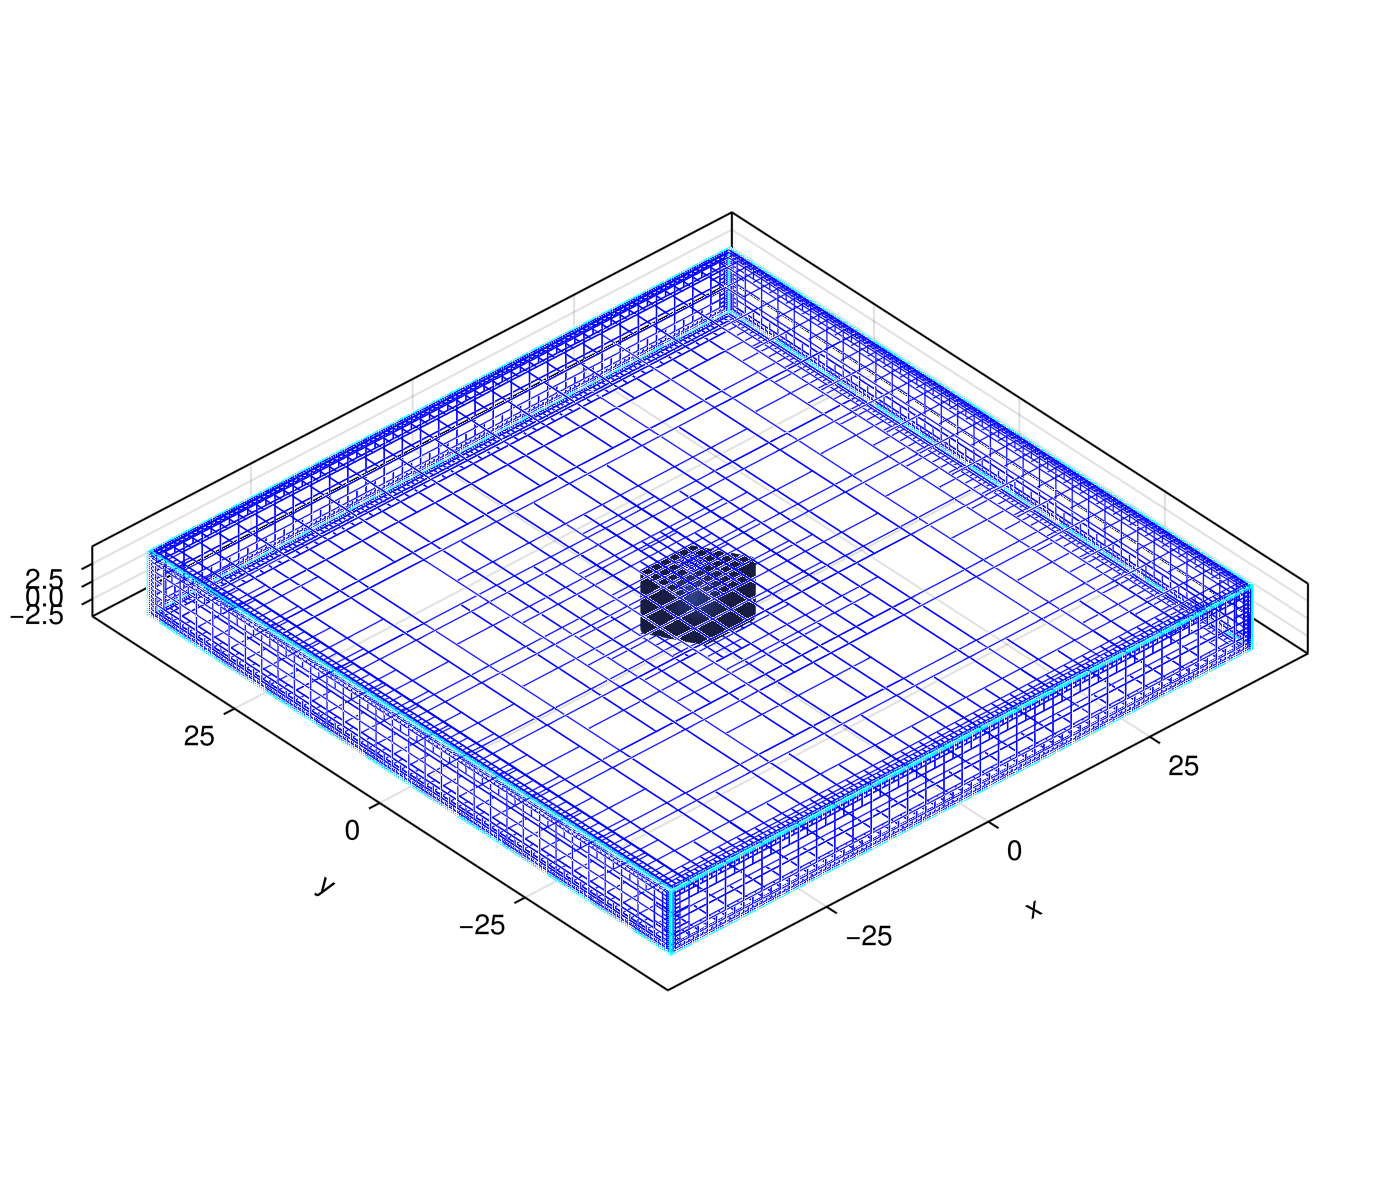
\includegraphics[width=\linewidth]{../codes/viz/figs/graphene_orbital_2.png}
    \end{subfigure}
    \caption{Orbital density and refined boundary panels for the graphene
        test case.}
    \label{fig:orbital-panels}
\end{figure}

\begin{figure}[htbp]
    \centering
    \begin{subfigure}[t]{0.4\textwidth}
        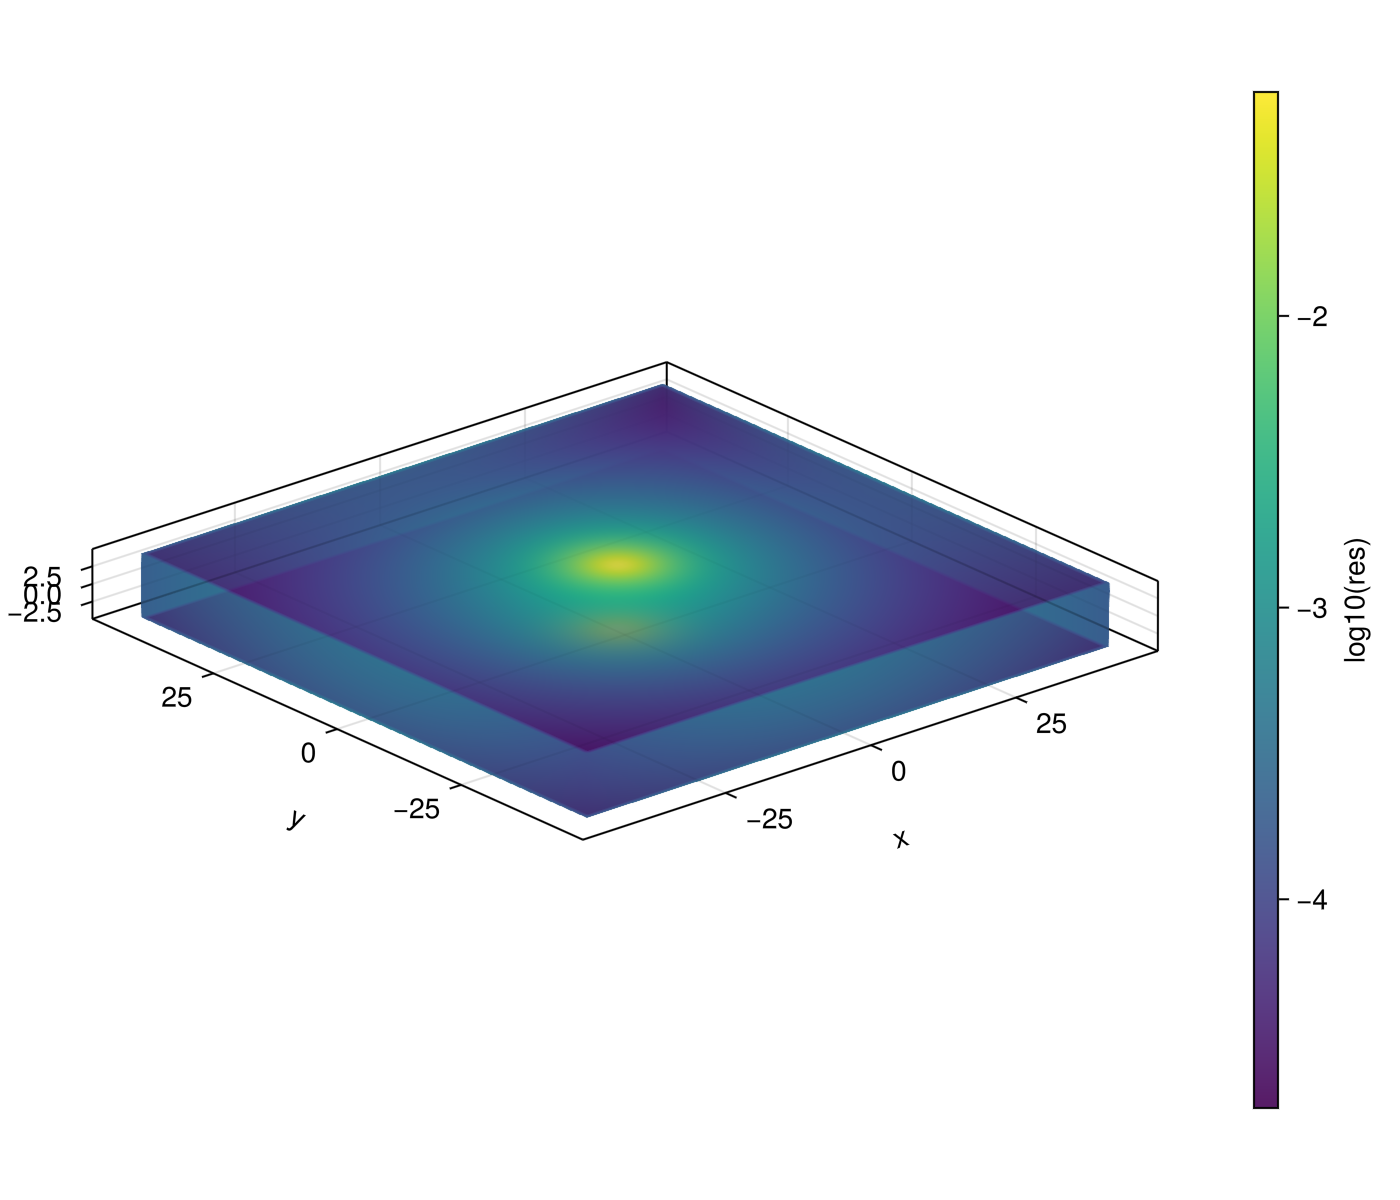
\includegraphics[width=\linewidth]{../codes/viz/figs/graphene_orbital_rhs.png}
    \end{subfigure}
    \begin{subfigure}[t]{0.4\textwidth}
        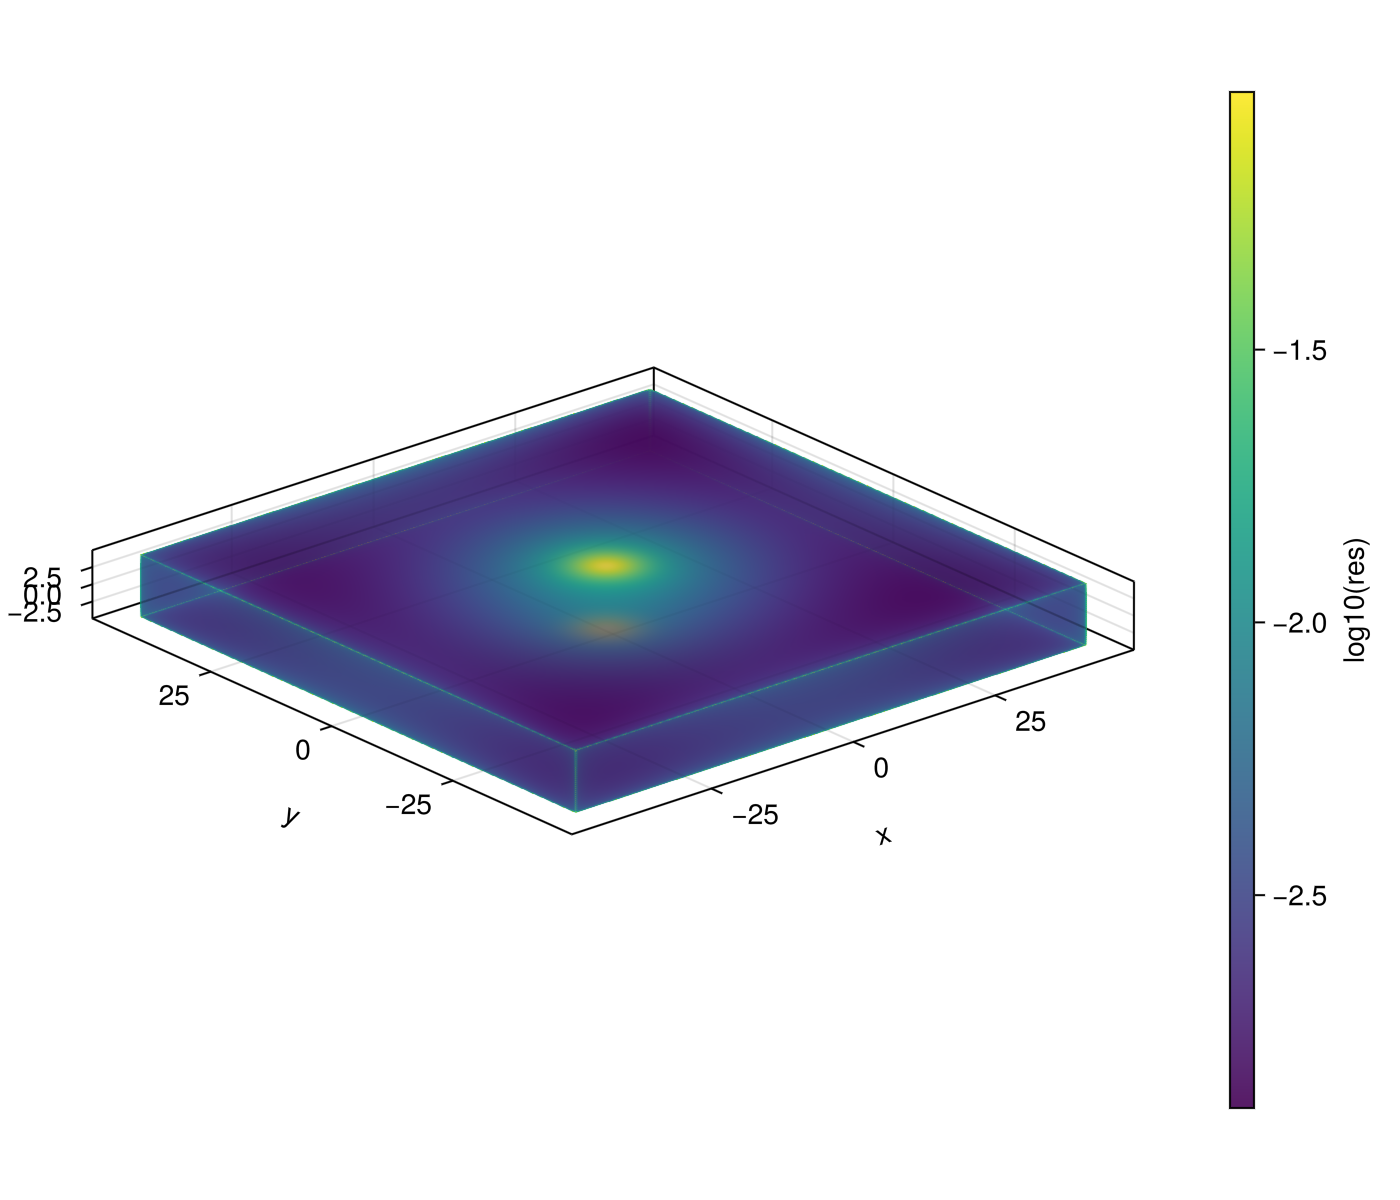
\includegraphics[width=\linewidth]{../codes/viz/figs/graphene_orbital_solution.png}
    \end{subfigure}
    \caption{Right-hand side $-\partial_{\V n} u_{\text{inc}}$ (left) and
        computed single-layer density $\sigma$ (right).}
    \label{fig:orbital-sol}
\end{figure}

\begin{figure}[htbp]
    \centering
    \includesvg[width=0.6\linewidth]{../codes/volume_source/figs/orbital_source_convergence.svg}
    \caption{Self-convergence of the evaluated potential at fixed points
        versus edge refinement $l_{\min}$ and quadrature order $p$.}
    \label{fig:orbital-conv}
\end{figure}

\subsection{Orbital densities crossing an interface}

For orbitals straddling a dielectric boundary, the sharp-interface screened
density has a slowly decaying Fourier transform; replacing the screening
function with a smooth $\text{erf}$-based transition restores rapid decay
suitable for the TKM--Fourier evaluator (Fig.~\ref{fig:screened-ft}).  The
decay in the $k_z$ direction is shown after $z$-upsampling in
Fig.~\ref{fig:kz-decay}.  Using the hybrid model (smooth $\epsilon$ for
$u_{\text{inc}}$, sharp interfaces for \eqref{eq:sl}) on graphene with
$L_x=L_y=90$~\AA, $L_z=2.8$~\AA, $\epsilon_r=2.4$, we compute the
Hubbard-model matrix elements $U_{00},U_{01},U_{02},U_{03}$ as defined in
Ref.~\cite{PhysRevLett.106.236805}.  The results agree well with the
constrained RPA data of that reference at small screening bandwidths
(Fig.~\ref{fig:hubbard}).  The current implementation already supports
multi-box slab geometries with refined edges, corners, and density-proximal
panels (Fig.~\ref{fig:multibox}).

\begin{figure}[htbp]
    \centering
    \includesvg[width=0.8\textwidth]{../codes/volume_source/figs/screened_gauss_ft.svg}
    \caption{Screened Gaussian with and without smoothing, and their
        Fourier transforms.  The smoothed (erf-based) screening decays
        rapidly, enabling TKM-Fourier evaluation.}
    \label{fig:screened-ft}
\end{figure}

\begin{figure}[htbp]
    \centering
    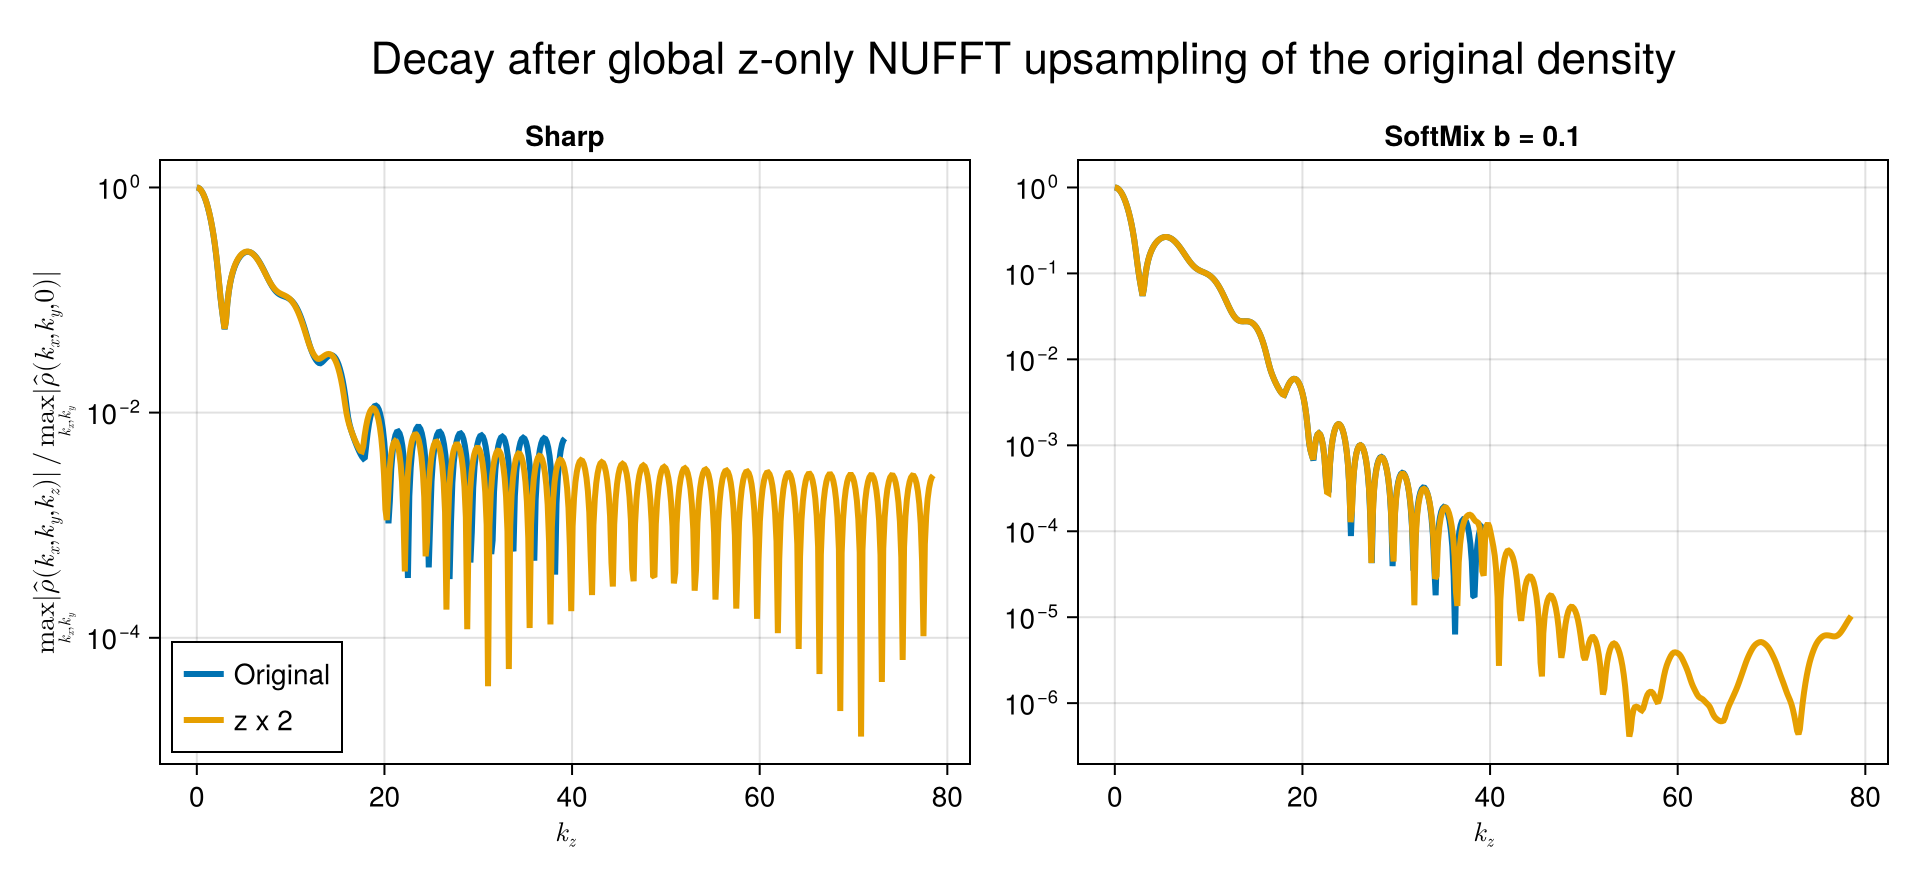
\includegraphics[width=0.6\textwidth]{../codes/graphene/figs/screened_density_kz_decay_z_upsampled.png}
    \caption{Fourier decay of the screened orbital density along $k_z$
        after $z$-upsampling, with and without smoothing.}
    \label{fig:kz-decay}
\end{figure}

\begin{figure}[htbp]
    \centering
    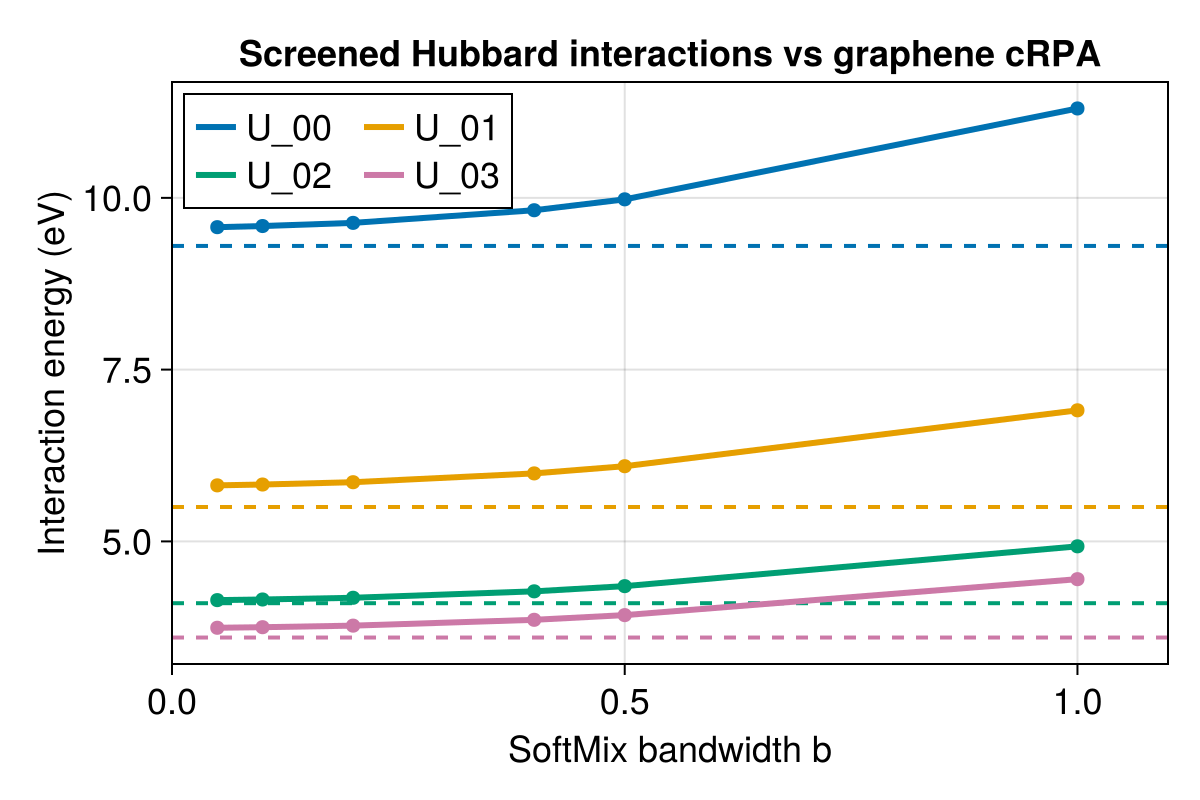
\includegraphics[width=0.5\textwidth]{../codes/graphene/figs/screened_hubbard_vs_crpa.png}
    \caption{Hubbard matrix elements $U_{00},U_{01},U_{02},U_{03}$ from
        the present solver (solid) versus the constrained RPA data of
        Ref.~\cite{PhysRevLett.106.236805} (dashed).}
    \label{fig:hubbard}
\end{figure}

\begin{figure}[htbp]
    \centering
    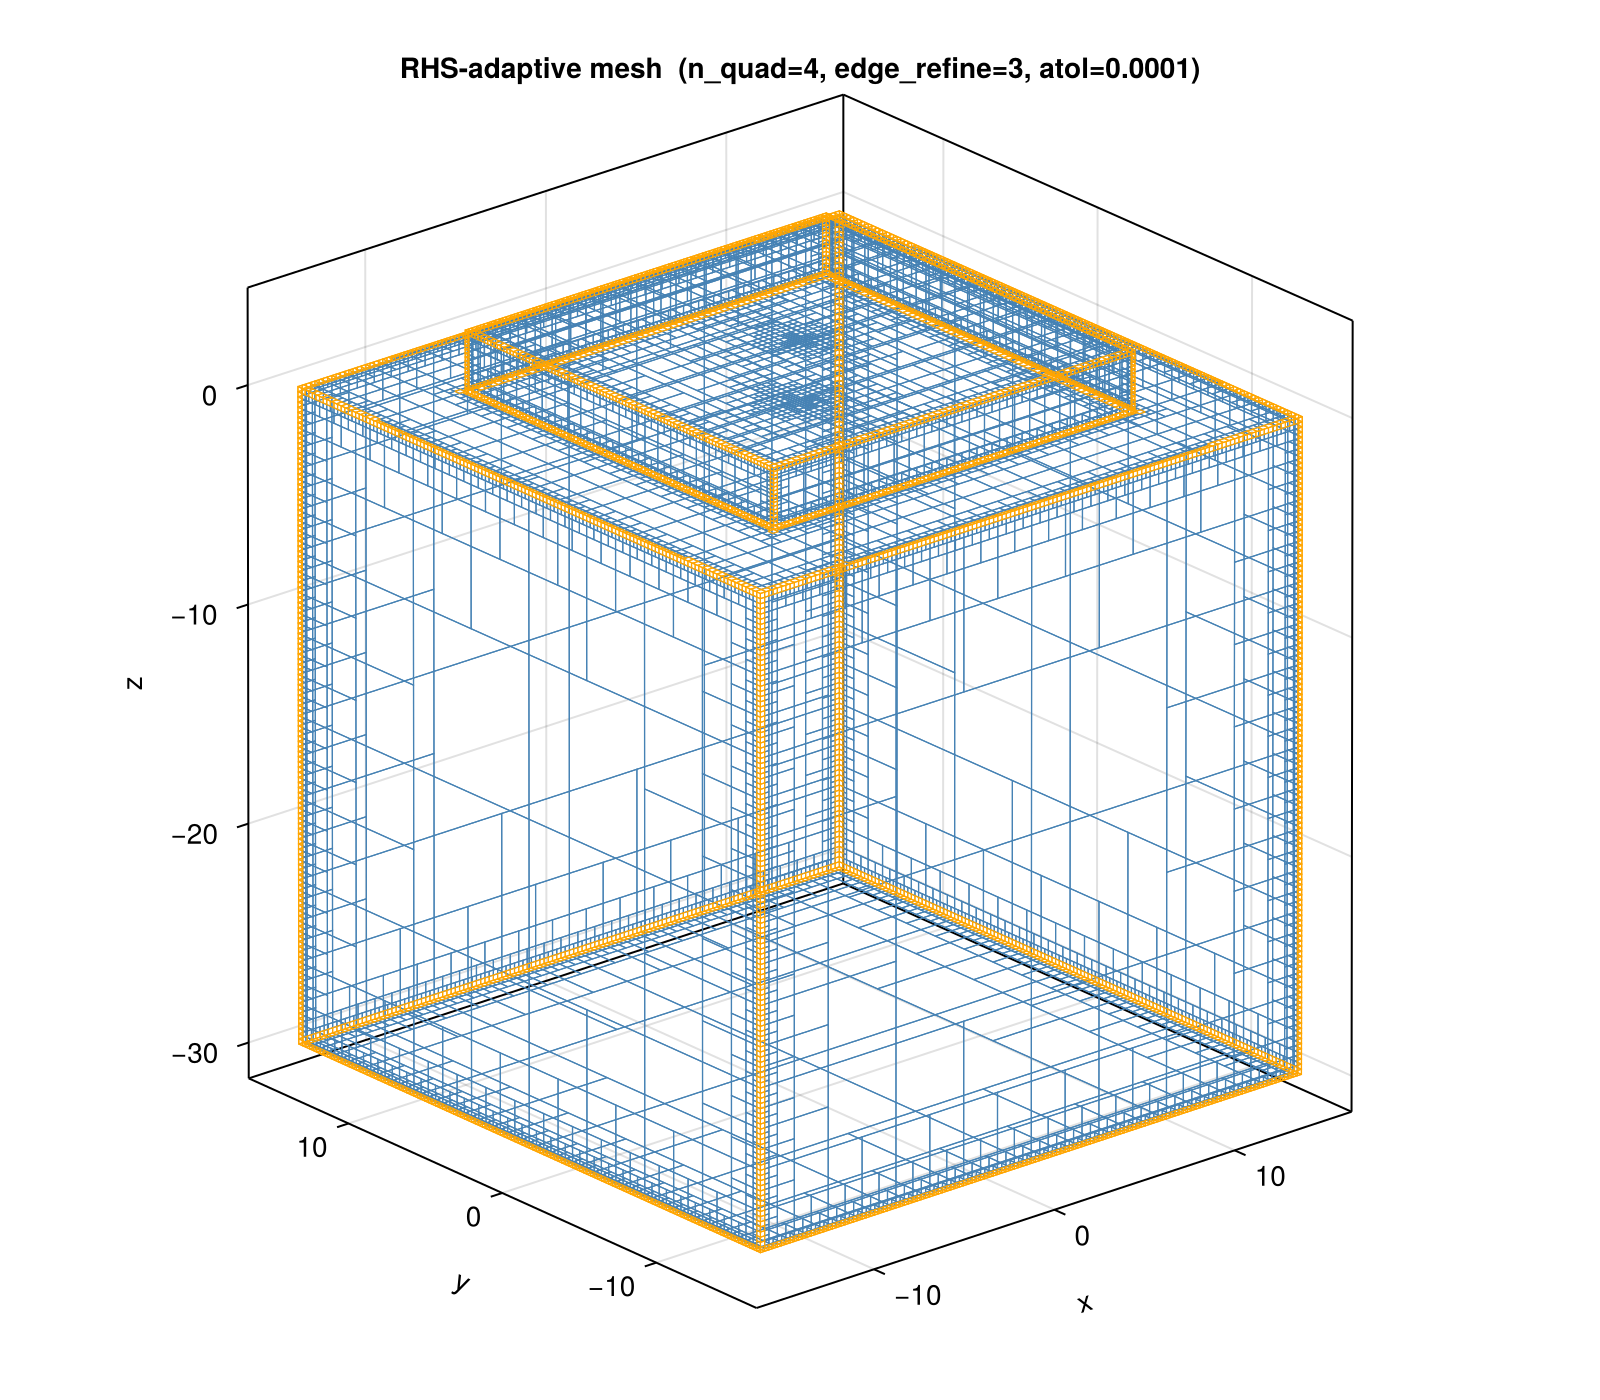
\includegraphics[width=0.6\textwidth]{../codes/multibox3d_convergence/figs/graphene_slab_rhs_mesh.png}
    \caption{Multi-box slab geometry with refined edge/corner (yellow) and
        density-proximal panels; the orbital density sits in the top slab.}
    \label{fig:multibox}
\end{figure}

\section{Summary}

We have developed an adaptive boundary-integral solver for the Poisson
equation with piecewise constant permittivity, targeted at the four-index
electron-repulsion integrals that drive correlated electronic structure.
The single-layer formulation gives a well-conditioned second-kind integral
equation away from the conductor limit; dyadic refinement at edges and
corners recovers the theoretically predicted corner singularities and
restores exponential convergence; Bernstein-ellipse estimates drive
upsampling-based near-field evaluation; and a hybrid smooth-$\epsilon$/
sharp-interface treatment handles orbital densities that cross material
boundaries.  On the graphene benchmark the method reproduces cRPA screened
Hubbard parameters from the literature, and the implementation already
supports multi-box slab geometries relevant to realistic 2D-material
heterostructures.

\bibliography{ref}

\end{document}
